\documentclass[10pt,journal,compsoc]{IEEEtran}

\usepackage[pdftex]{graphicx}    
\usepackage{cite}
\hyphenation{op-tical net-works semi-conduc-tor}


\begin{document}

\title{Deep Learning for Fruit Classification}

\author{Vijayasri Iyer}

\markboth{Inference project, Robotics Nanodegree, Udacity}%
{}
\IEEEtitleabstractindextext{%

\begin{abstract}
This paper presents a novel use case for GoogLeNet, a popular convolutional network architecture, for classifying fruits. This application forms the basis for a kitchen service robot to develop relevant scene understanding capabilities using deep learning. The model performs with an accuracy of 50 percent in the above classifiation, which makes it a good candidate for a commercially viable product.\end{abstract}

% Note that keywords are not normally used for peerreview papers.
\begin{IEEEkeywords}
NVIDIA DIGITS, GoogLeNet, Deep learning.
\end{IEEEkeywords}}


\maketitle
\IEEEdisplaynontitleabstractindextext
\IEEEpeerreviewmaketitle
\section{Introduction}
\label{sec:introduction}

\IEEEPARstart{T}{he} three main qualities of a robot are perception, decision-making and actuation. For a kitchen service robot, it has to recognize the relevant objects in the scene, understand the action to be taken, and then interact with the real-world objects to perform the action. This paper aims to solve the first of three problems in implementing this robot, which had become quite easy with the rise of deep learning algorithms. Here GoogLeNet, a commercially available deep convolutional net architecture is used to classify fruit. Fruit classification is used a basis to create a model that ultimately classifies all types of kitchen items and foods with ease.

\section{Background / Formulation}
The NVIDIA DIGITS interface was used to train the GoogLe Net model on both, the custom as well as the supplied data set. DIGITS simplifies the common deep learning tasks such as managing data, training neural nets on Multi-GPU systems, monitoring performance in real-time and selecting the best performing model for deployment. GoogLeNet, is a 22-layer convolutional network, which won the IMAGENET 2014 challenge with an extremely low error margin of 6.66 percent, thus outperforming humans in image recognition tasks \cite{googlenet}. The notable part about this network is that it uses inception modules instead of regular convolutional layers. An inception module computes multiple different transformations over the same input map in parallel, concatenating their results into a single output. A schematic of the inception layer is shown in fig 1. 


%example for inserting image
\begin{figure}[thpb]
      \centering
      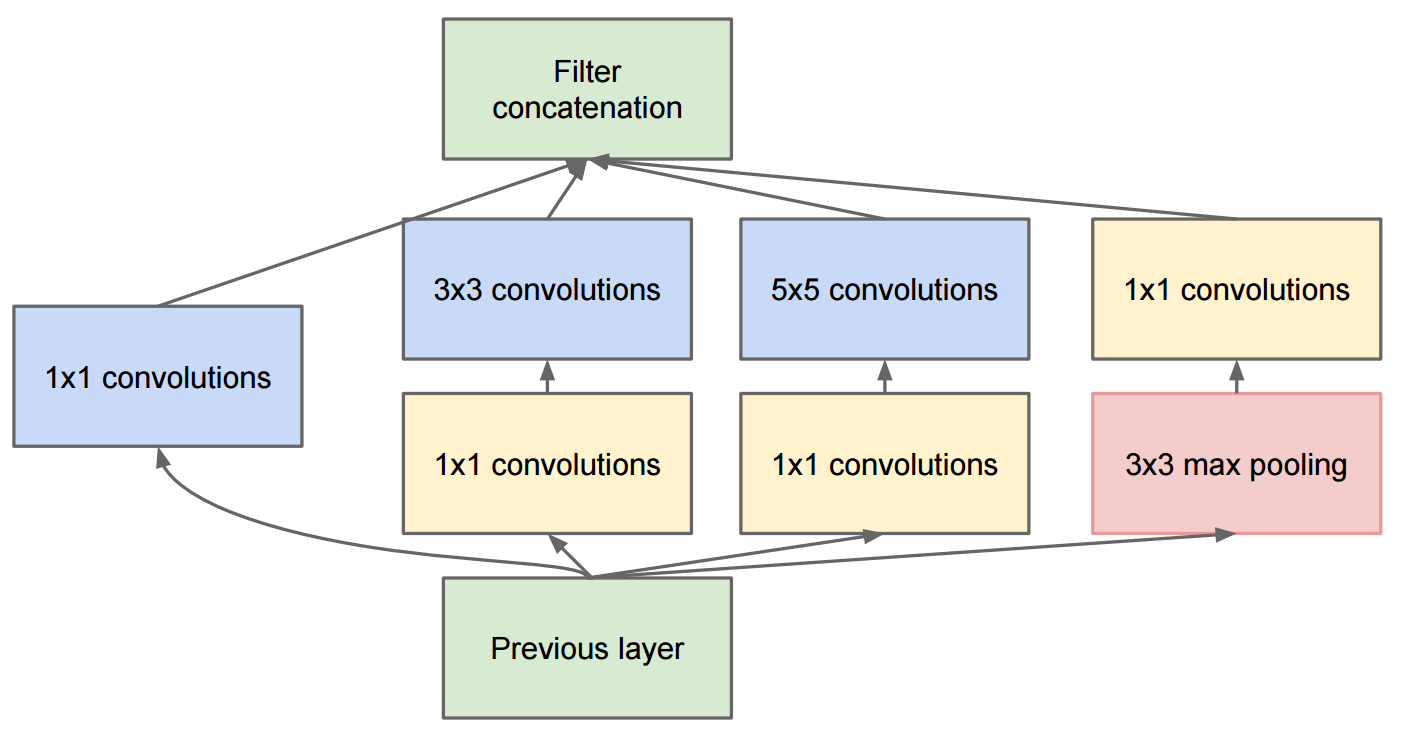
\includegraphics[width=\linewidth]{inc.png}
      \caption{Inception Module.}
      \label{fig:robot1}
\end{figure}

GoogLeNet inception modules consist of convolutional, maxpooling as well as average pooling layers. The GoogLeNet model has 4 million parameters in total. Hence this model is easier to maintain and gives a better overall result than other popular networks such as AlexNet, LeNet. However, the training time is comparatively longer, which makes it better suited to smaller data sets, especially if time is a constraint. It accepts images of type RGB (3-channels) and dimensions 256x256 pixels. The architecture of GoogLeNet is shown in fig 2.

%example for inserting image
\begin{figure}[thpb]
      \centering
      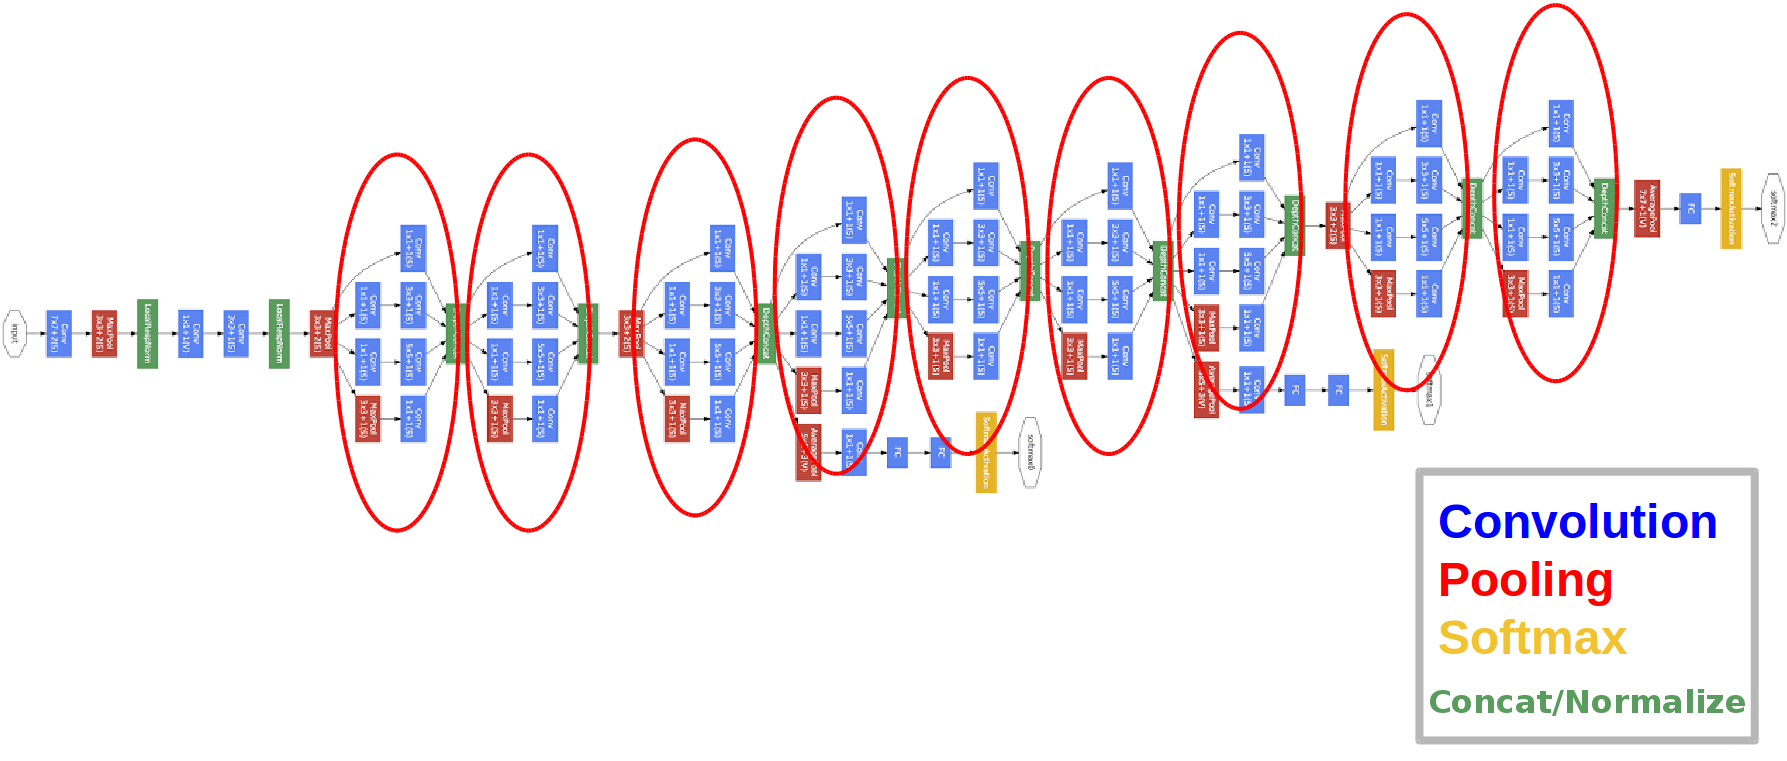
\includegraphics[width=\linewidth]{goog.png}
      \caption{Architecture of GoogLeNet.}
      \label{fig:robot1}
\end{figure}


\section{Data Acquisition}
The data set used in this paper is a subset of the Fruits360 data set available on Kaggle. While the original data set consists of 60 fruits and 38409 images, the classification task used 4 classes with around 440-500 images each for training and validation. The training data was further split into separate training and validation sets by the DIGITS interface.
The testing images captured using a Samsung smartphone camera and consisted of 4 images per class. The categories in  the dataset are Banana, Apple, Orange and Papaya. A few sample images from the data set are shown in fig 3, whereas the sample images from the testing set can be seen in fig 6.

%example for inserting image
\begin{figure}[thpb]
      \centering
      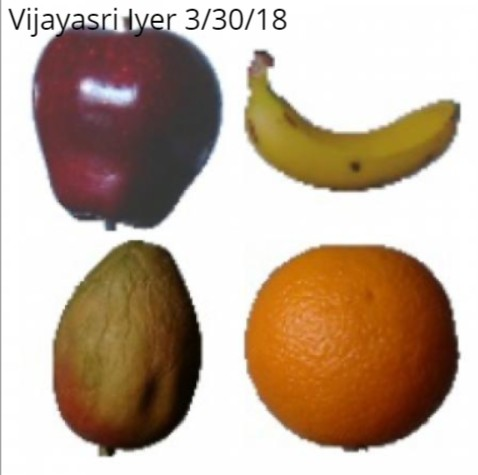
\includegraphics[width=\linewidth]{col.png}
      \caption{Fruit data set images.}
      \label{fig:robot1}
\end{figure}

The NVIDIA digits was evaluated with a sample data set, before training with the above data. This sample data set consists of 3 categories : bottles, candy-boxes and nothing. The total number of images in the data set is 7750, which was split into training, validation and testing sets by the DIGITS interface. Sample images from the supplied data set are shown below in fig 4.

%example for inserting image
\begin{figure}[tbhp]
      \centering
      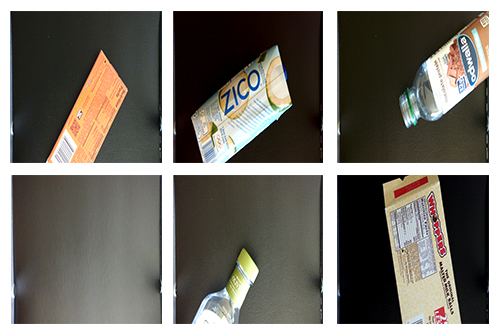
\includegraphics[width=\linewidth]{data.jpg}
      \caption{Sample data set images.}
      \label{fig:robot1}
\end{figure}

\section{Results}
The results of the training and evaluation are discussed in the following two sections.

\subsection{DIGITS Sample Data}
This data was trained on GoogLeNet for 15 epochs, with a batch size of 64 and learning rate of 0.01. The model achieved a final accuracy of 75.4 percent in the testing phase. The results of running the evaluate in the DIGITS workspace terminal can be seen below in fig 5.

%example for inserting image
\begin{figure}[tbhp]
      \centering
      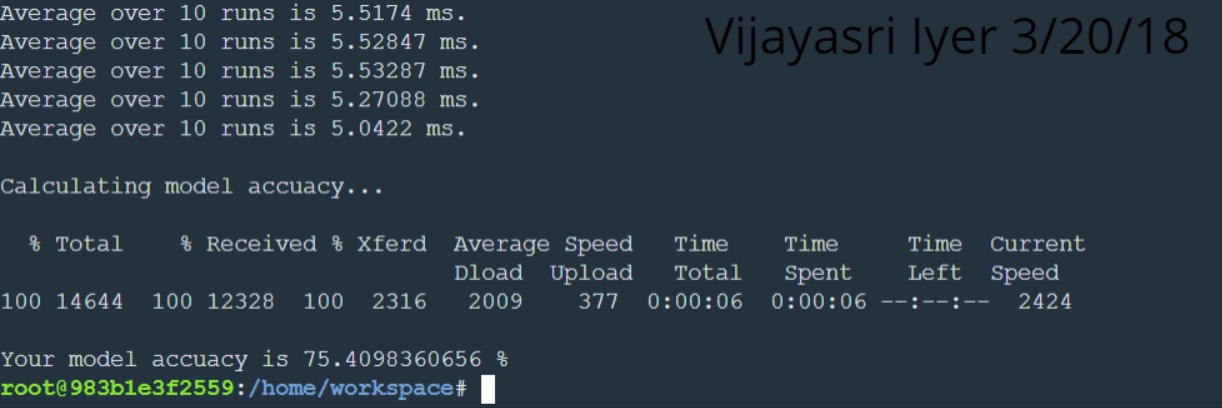
\includegraphics[width=\linewidth]{res.png}
      \caption{Sample data set images.}
      \label{fig:robot1}
\end{figure}

The average inference time of the model is 5ms which is sufficiently high to be deployed on hardware for real-time testing.


\subsection{Fruit Classification Data}
This data was trained for 30 epochs, with a batch size of 32 and learning rate 0.01. The training accuracy of the model was nearly 70 percent. But, model achieved a training accuracy of only 50, which means it misclassified half the images, and the confidence score of the correctly classified images was only a little above 35 percent.

%example for inserting image
\begin{figure}[tbhp]
      \centering
      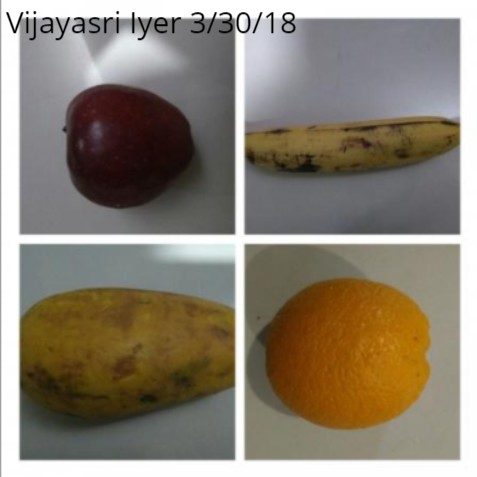
\includegraphics[width=\linewidth]{test.png}
      \caption{Sample testing images.}
      \label{fig:robot1}
\end{figure}

\section{Discussion}
As one can infer from the above sections, the Fruit classification model has a relaatively low accuracy while training as well as in the testing phase. Hence, there is reason to believe that the model may be overfitting. The reasons for this could be the nature of data set, where all the fruit images consist of a white background and that the training dataset is augmented by rotating the object by a certain angle to create more data. One of the problems with using the GoogLeNet for such a task is that, the nature of this task maybe to simple for such a complex architecture. Also, since this model is to deployed in an indoor environment, the accuracy of this model is more important than the inference timing. In this case, the task isn't urgent in nature so an increase in inference timing won't affect the performance of the product that will eventually use the model.

\section{Conclusion / Future work}
This Fruit classifier system, was an attempt to making an end-to-end system that can recognize all kinds of different kitchen and food items. This could then be implemented on a kitchen service robot, which gives it full-understanding of the environment around. This product can be made commercially viable, but with some changes to the model which may improve the overall accuracy. To extend this project, various aspects can be improved. This may include increasing the number of categories, or getting a different dataset that covers more items to be classified Another option may be to choose a different network architecture for the following architecture which might be better suited to the purpose. 


\bibliography{ref}
\bibliographystyle{ieeetr}
\end{document}